% ---------------------------------------------------------------
% Preamble
% ---------------------------------------------------------------
%\documentclass[a4paper,fleqn,longmktitle]{cas-sc}
\documentclass[a4paper,fleqn]{cas-dc}
%\documentclass[a4paper]{cas-dc}
%\documentclass[a4paper]{cas-sc}
% ---------------------------------------------------------------
% Make margins bigger to fit annotations. Use 1, 2 and 3. TO be removed later
%\paperwidth=\dimexpr \paperwidth + 6cm\relax
%\oddsidemargin=\dimexpr\oddsidemargin + 3cm\relax
%\evensidemargin=\dimexpr\evensidemargin + 3cm\relax
%\marginparwidth=\dimexpr \marginparwidth + 3cm\relax
% -------------------------------------------------------------------- 
% Packages
% --------------------------------------------------------------------
% Figure packages
\usepackage{graphicx}
\usepackage{float}
\restylefloat{table}
\usepackage{adjustbox}
% Text, input, formatting, and language-related packages
\usepackage[T1]{fontenc}
\usepackage{subcaption}

\usepackage{csvsimple}

% TODO package
\usepackage[bordercolor=gray!20,backgroundcolor=blue!10,linecolor=black,textsize=footnotesize,textwidth=1in]{todonotes}
\setlength{\marginparwidth}{1in}
% \usepackage[utf8]{inputenc}
% \usepackage[nomath]{lmodern}

% Margin and formatting specifications
%\usepackage[authoryear]{natbib}
\usepackage[sort]{natbib}
\setcitestyle{square,numbers}

 %\bibliographystyle{cas-model2-names}

\usepackage{setspace}
\usepackage{subfiles} % Best loaded last in the preamble

% \usepackage[authoryear,longnamesfirst]{natbib}

% Math packages
\usepackage{amsmath, amsthm, amssymb, amsfonts, bm, nccmath, mathdots, mathtools, bigints, ulem}

\usepackage{tikz}
\usepackage{pgfplots}
\usetikzlibrary{shapes.geometric,angles,quotes,calc}

\usepackage{placeins}

\usepackage[final]{pdfpages}

\usepackage{numprint}

% --------------------------------------------------------------------
% Packages Configurations
\usepackage{enumitem}
% --------------------------------------------------------------------
% (General) General configurations and fixes
\AtBeginDocument{\setlength{\FullWidth}{\textwidth}}	% Solves els-cas caption positioning issue
\setlength{\parindent}{20pt}
%\doublespacing
% --------------------------------------------------------------------
% Other Definitions
% --------------------------------------------------------------------
\graphicspath{{Figures/}}
% --------------------------------------------------------------------
% Environments
% --------------------------------------------------------------------
% ...

% --------------------------------------------------------------------
% Commands
% --------------------------------------------------------------------

% ==============================================================
% ========================== DOCUMENT ==========================
% ==============================================================
\begin{document} 
%  --------------------------------------------------------------------

% ===================================================
% METADATA
% ===================================================
\title[mode=title]{Supercritical fluid extraction of essential oil from chamomile flowers: modelling and parameter estimation}                      
\shorttitle{Supercritical fluid extraction of essential oil from chamomile flowers: modelling and parameter estimation}

\shortauthors{OS, PO}

\author[1]{Oliwer Sliczniuk}[orcid=0000-0003-2593-5956]
\ead{oliwer.sliczniuk@aalto.fi}
\cormark[1]
\credit{a}

\author[1]{Pekka Oinas}[orcid=0000-0002-0183-5558]
\credit{b}

\address[1]{Aalto University, School of Chemical Engineering, Espoo, 02150, Finland}
%\address[2]{2}

\cortext[cor1]{Corresponding author}

% ===================================================
% ABSTRACT
% ===================================================
\begin{abstract}
This study investigates the supercritical extraction process of essential oil from chamomile flowers. Essential oils of chamomile are used extensively for medicinal purposes. Many different chamomile products have been developed, the most popular of which is herbal tea. In this study, a mathematical model is formulated that describes the governing mass transfer phenomena in a solid-fluid environment under supercritical conditions using carbon dioxide. The concept of quasi-one-dimensional flow is applied to reduce the number of spatial dimensions. The flow of carbon dioxide is assumed to be uniform across any cross-section, although the area available for the fluid phase can vary along the extractor. The physical properties of the solvent are estimated based on the Peng-Robinson equation of state. Model parameters, including the partition factor, internal diffusion coefficient and decaying factor, were determined through maximum likelihood estimation based on experimental data assuming normally distributed errors. A set of laboratory experiments was performed under multiple constant operating conditions: $30-40~^\circ$C, $100-200$ bar and $3.33-6.67 \cdot 10^{-5}$ kg/s.

%A distributed-parameter model describes the fluid-solid extraction process.

\end{abstract}

\begin{keywords}
Supercritical extraction \sep Parameter estimation \sep Mathematical modelling
\end{keywords}

% ===================================================
% TITLE
% ===================================================
\maketitle

% ===================================================
% Section: Introduction
% ===================================================

\section{Introduction}

This study investigates the extraction of essential oil from chamomile flowers (Matricaria chamomilla L.) via supercritical fluid extraction techniques and the modelling of this process. Chamomile is a medicinal herb widely cultivated in southern and eastern Europe — in countries such as Germany, Hungary, France and Russia. It can be found outside Europe, for instance in Brazil as discussed by \citet{Singh2011}. This plant is distinguished by its hollow, bright gold cones, housing disc or tubular florets and surrounded by about fifteen white ray or ligulate florets. Chamomile has been used for its medicinal benefits, serving as an anti-inflammatory, antioxidant, mild astringent, and healing remedy. Aqueous extract of chamomile is widely used to calm nerves and mitigate anxiety, hysteria, nightmares, insomnia and other sleep-related conditions, according to \citet{Srivastava2009}. \citet{Orav2010} reported that oil yields from dried chamomile samples ranged from 0.7 to 6.7 mL/kg. The highest yields of essential oil, between 6.1 and 6.7 mL/kg, were derived from chamomile sourced from Latvia and Ukraine. In comparison, chamomile from Armenia exhibited a lower oil content of 0.7 mL/kg.

Evaluating the economic viability of the process is essential when choosing a suitable technology for essential oil extraction. Traditional methods, such as distillation and organic solvent extraction, are commonly employed but have drawbacks. Distillation, for example, involves high temperatures that can lead to the thermal degradation of heat-sensitive compounds. This limitation has led to the increased popularity of alternative techniques such as supercritical fluid extraction. Supercritical carbon dioxide is appealing thanks to its distinctive properties: it is inflammable, non-toxic and non-corrosive. Supercritical fluids can exhibit both gas- and liquid-like properties, allowing for adjustable dissolving power through changes in operating conditions.

The literature offers various mathematical models to describe the extraction of valuable compounds from biomass. Selecting a process model is case-to-case dependent and requires analysis of each model's specific assumptions about mass transfer and thermodynamic equilibrium.

The model proposed by \citet{Reverchon1993} is called the hot ball model, as it is based on an analogy to heat transfer and describes an extraction process from solid particles. This model assumes that particles contain low quantities of solute and that solubility is not a limiting factor.

The Broken-and-Intact Cell model, proposed by \citet{Sovova1994}, assumes that external surfaces of particles are mechanically disrupted, allowing the solvent access to the solute in the broken cells. In contrast, the solute in intact cells remains less accessible due to higher mass transfer resistance.

\citet{Reverchon1996} formulated a fluid-solid extraction model where the solute is treated as a single component, governed by internal mass transfer resistance and omitting the effects of external mass transfer, axial dispersion and variations in fluid density and flow rate throughout the bed.

This work builds upon the linear kinetic model suggested by \citet{Reverchon1996}, deriving fundamental governing equations to develop a comprehensive model for the chamomile oil extraction process. This model aims for control-oriented simplicity, assuming a semi-continuous operation within a cylindrical vessel. The process involves a supercritical solvent being pumped through a fixed bed of finely chopped biomass to extract the solute, followed by separation of the solvent and solute in a flush drum to collect the extract. Parameters such as pressure ($P$), feed flow rate ($F_{in}$) and inlet temperature ($T_{in}$) are adjustable and measurable, while the outlet temperature ($T_{out}$) and the amount of product at the outlet can only be monitored. Figure \ref{fig: SFE_drawing} presents a simplified process flow diagram.

\begin{figure}[h!]
	\centering
	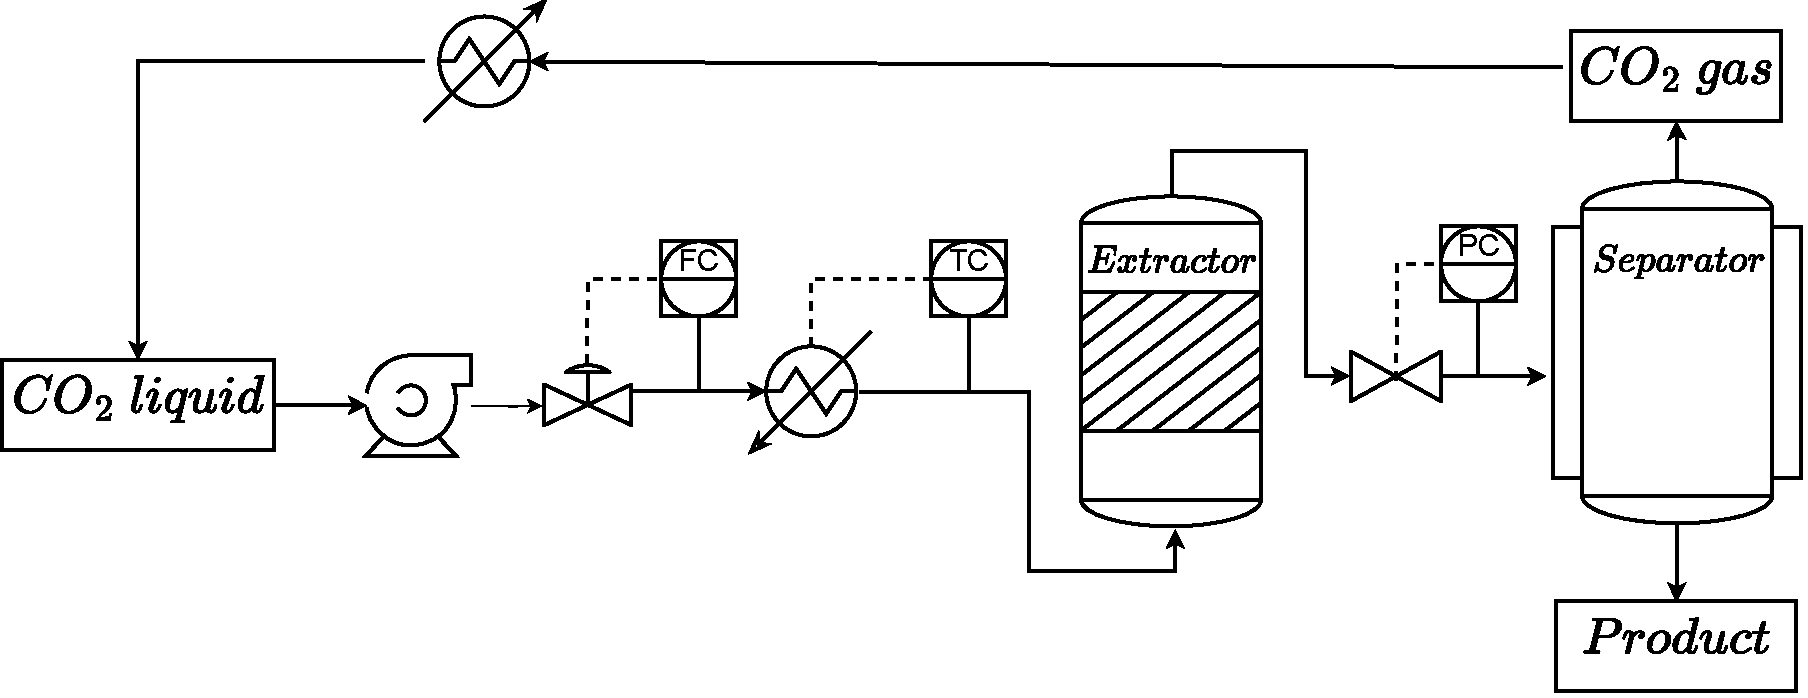
\includegraphics[width=\columnwidth]{Figures/PFD.drawio.pdf}
	\caption{Process flow diagram.}
	\label{fig: SFE_drawing}
\end{figure}

This study focuses on finding a process model for the extraction of natural substances from solid materials using supercritical fluids, with a particular emphasis on supercritical CO$_2$. The approach involves estimating the solvent properties through thermodynamic relationships and determining the extraction kinetic parameters via a series of experiments conducted under various conditions. Maximum likelihood estimation is employed to solve the parameter estimation problem. Later, the correlations between parameters and operating conditions are proposed.

% ===================================================
% Section: Methods
% ===================================================

\section{Materials and methods} \label{CH: Materials and methods}

\subsection{Governing equations} \label{CH:Governing_equations_chapter}
Following the work of \citet{Anderson1995}, the governing equations for a quasi-one-dimensional flow were derived. A quasi-one-dimensional flow refers to a fluid flow scenario assuming that the flow properties are uniformly distributed across any cross-section. This simplification is typically applied when the flow channel's cross-sectional area changes, such as through irregular shapes or partial filling of an extractor. According to this assumption, velocity and other flow properties change solely in the flow direction.

As discussed by \citet{Anderson2023}, all flows are compressible, but some of them can be treated as incompressible when the Mach number is smaller than 0.3. This assumption leads to the incompressible condition: $\nabla \cdot u =0$, which is valid for constant density (strict incompressible) or varying density flow. The assumption allows for removing acoustic waves and large perturbations in density and/or temperature. In the 1-D case, the incompressibility condition becomes $\frac{du}{dz} = 0$, so the fluid velocity is constant.

The set of quasi-one-dimensional governing equations in Cartesian coordinates is described by Equations \ref{EQ: CompressibleEuler_1} - \ref{EQ: CompressibleEuler_3}:

{\footnotesize
	\begin{align}
		\label{EQ: CompressibleEuler_1}
		\cfrac{\partial \left( \rho_f A_f \right) }{\partial t} + \cfrac{\partial \left( \rho_f A_f v \right)}{\partial z} &= 0 \\
		\cfrac{\partial \left( \rho_f v A_f \right) }{\partial t} + \cfrac{\partial \left( \rho_f A_f v^2 \right)}{\partial z} &= -A_f \cfrac{\partial P}{\partial z} \label{EQ: CompressibleEuler_2} \\
		\cfrac{\partial \left( \rho_f e A_f \right) }{\partial t} + \cfrac{\partial \left( \rho_f A_f v e\right)}{\partial z} &= -P\cfrac{\left( A_f v \right)}{\partial z} + \cfrac{\partial}{\partial z} \left( k \cfrac{\partial T}{\partial z} \right)   
		\label{EQ: CompressibleEuler_3}
	\end{align}  
}

where $\rho_f$ is the density of the fluid, $A_f$ is the function which describes a change in the cross-section, $v$ is the velocity, $P$ is the total pressure, $e$ is the internal energy of the fluid, $t$ is time and $z$ is the spatial direction.

\subsection{Extraction model} \label{CH: Extraction_model}
\subsubsection{Continuity equation} \label{CH: Continuity}

The previously derived quasi-one-dimensional continuity equation (Equation \ref{EQ: CompressibleEuler_1}) is redefined by incorporating the function $A_f = A\phi$. This modification distinguishes constant and varying terms, where the varying term accounts for changes in the cross-sectional area available for the fluid. Equation \ref{EQ: Continuity_differential} shows the modified continuity equation:

{\footnotesize
	\begin{equation} \label{EQ: Continuity_differential}
		\frac{\partial (\rho_f \phi)}{\partial t} + \frac{\partial (\rho_f v A\phi)}{\partial z} = 0
	\end{equation}
}
where $A$ is the total cross-section of the extractor and $\phi$ describes porosity along the extractor.

Assuming that the mass flow rate is constant in time, the temporal derivative becomes the mass flux F, and the spatial derivative can be integrated along $z$ as

{\footnotesize
	\begin{equation}
		\int \frac{\partial (\rho_f v A \phi )}{\partial z} dz = F \rightarrow F=\rho_f v A\phi
	\end{equation}
}

To simplify the system dynamics, it is assumed that $F$ is a control variable and affects the whole system instantaneously (due to $\nabla \cdot u = 0$), which allows finding the velocity profile that satisfies mass continuity based on $F$, $\phi$ and $\rho_f$:

{\footnotesize
	\begin{equation} \label{EQ:Velocity_1}
		v = \cfrac{F}{\rho_f A\phi} 
	\end{equation}
}

Similarly, superficial velocity may be introduced:

{\footnotesize
	\begin{equation} \label{EQ:Velocity_2}
		u = v \phi = \cfrac{F}{\rho_f A }
	\end{equation}
}

The fluid density $\rho_f$ can be obtained from an equation of state (Appendix \ref{subsubsec: Equation of state}) if the temperature and thermodynamic pressure are known along $z$. Variation in fluid density may occur due to pressure or inlet temperature changes. In a non-isothermal case, in Equations \ref{EQ:Velocity_1} and \ref{EQ:Velocity_2} $\rho_f$ is considered the average fluid density along the extraction column.

\subsubsection{Mass balance for the fluid phase} \label{CH: Mass_balance_fluid}

Equation \ref{Model_fluid} describes the movement of the solute in the system, which is constrained to the axial direction due to the quasi-one-dimensional assumption. Given that the solute concentration in the solvent is negligible, the fluid phase is described as pseudo-homogeneous, with properties identical to those of the solvent itself. It is also assumed that the thermodynamic pressure remains constant throughout the device. The analysis further simplifies the flow dynamics by disregarding the boundary layer near the extractor's inner wall. This leads to a uniform velocity profile across any cross-section perpendicular to the axial direction. Thus, the mass balance equation includes convection, diffusion and kinetic terms representing the fluid phase behaviour:

{\footnotesize
	\begin{equation}
		\label{Model_fluid}
		\frac{\partial c_f}{\partial t}
		+ \frac{1}{\phi} \frac{\partial \left( c_f u\right)}{\partial z}
		= \frac{1-\phi}{\phi} r_e
		+ \frac{1}{\phi} \frac{\partial}{\partial z} \left( D^M_e \frac{\partial c_f}{\partial z} \right)
	\end{equation}
}

where $c_f$ represents the solute concentration in the fluid phase, $r_e$ is the mass transfer kinetic term and $D^M_e$ is the axial diffusion coefficient.

\subsubsection{Mass balance for the solid phase} \label{Mass_balance_solid}

As given by Equation \ref{Model_solid}, the solid phase is considered stationary, without convection and diffusion terms in the mass balance equation. Therefore, the only significant term in this equation is the kinetic term of Equation \ref{Model_kinetic_basic}, which connects the solid and fluid phases. For simplicity, the extract is represented by a single pseudo-component: 

{\footnotesize
	\begin{equation} 
		\label{Model_solid}
		%		{\scriptsize\begin{equation}
				\cfrac{\partial c_s}{\partial t} = \underbrace{ r_e }_{\text{Kinetics}}
		\end{equation} }
		
		\subsubsection{Kinetic term} \label{CH: Kinetic}
		
		As the solvent flows through the bed, CO$_2$ molecules diffuse into the pores and adsorb on the particle surface to form an external fluid film around the solid particles due to the solvent-solid matrix interactions. The dissolved solute diffuses from the particle's core through the solid-fluid interface, the pore and the film into the bulk. Figure \ref{fig: SFE_Mechanism} shows the mass transfer mechanism, where the mean solute concentration in the solid phase is denoted as $c_s$, and the equilibrium concentrations at the solid-fluid interface are denoted as $c_s^*$ and $c_p^*$ for the solid and fluid phases, respectively. The concentration of the solutes in the fluid phase in the centre of the pore is denoted as $c_p$. As the solute diffuses through the pore, its concentration changes and reaches $c_{pf}$ at the pore opening. Then, the solute diffuses through the film around the particle and reaches bulk concentration $c_f$. The two-film theory describes the solid-fluid interface inside the pore. The overall mass transfer coefficient can be determined from the relationship between the solute concentration in one phase and its equilibrium concentration.
		
		\begin{figure}[h!]
			\centering
			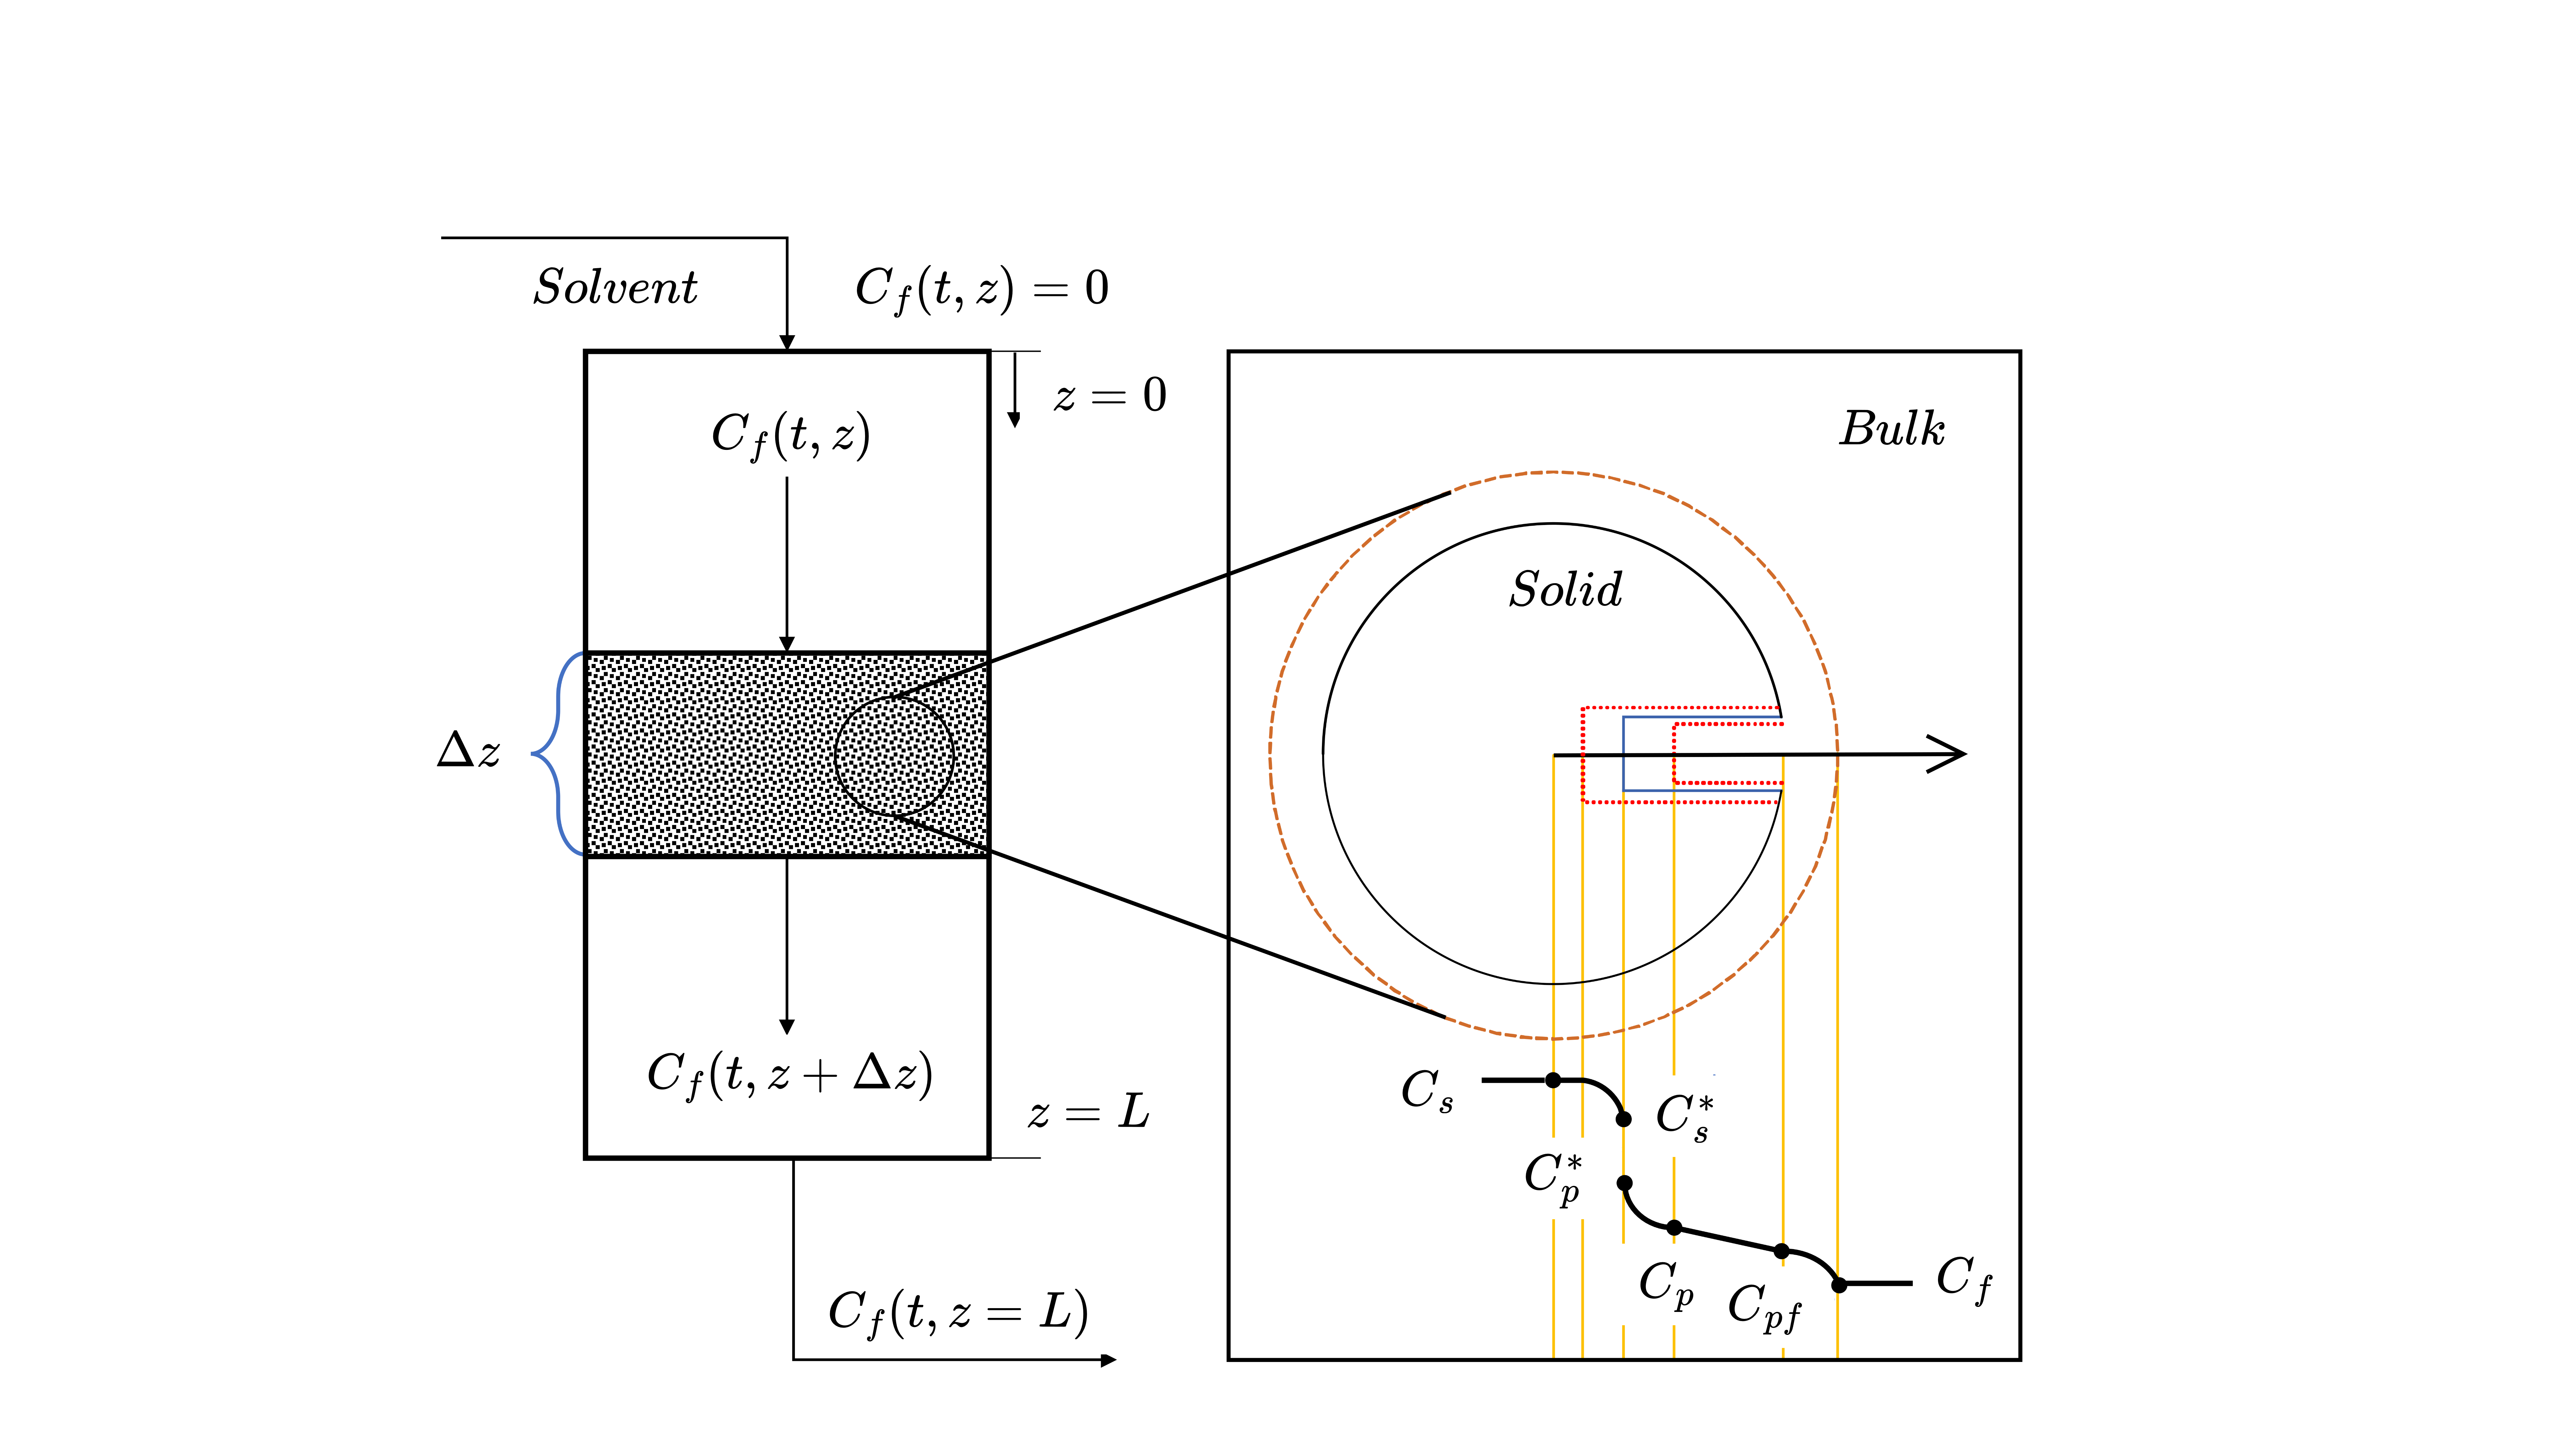
\includegraphics[trim = 45cm 0cm 60cm 20cm,clip,width=0.85\columnwidth]{Figures/SFE_PFD.drawio.png}	
			\caption{Mass transfer mechanism.}
			\label{fig: SFE_Mechanism}
		\end{figure}
		
		\citet{Bulley1984} suggest a process where the driving force for extraction is given by the difference between the concentration of the solute in the bulk, $c_f$, and in the centre of the pore, $c_p^*$. The concentration $c_p^*$ is in equilibrium with $c_s$ according to the equilibrium relationship. The rate of extraction is thus $r_e\left(c_f - c^*_p(c_s)\right)$. In contrast, \citet{Reverchon1996} proposes a driving force given by the difference between $c_s$ and $c_p^*$. Concentration $c_p^*$ is determined by the equilibrium relationship with $c_f$ and the extraction rate given by Equation \ref{Model_kinetic_basic}:
		
		{\footnotesize
			\begin{equation} \label{Model_kinetic_basic}
				r_e = \cfrac{D_i}{\mu l^2 }\left(c_s - c_p^* \right)
		\end{equation} }
		
		where $\mu$ is sphericity, $l$ a characteristic dimension of particles that can be defined as $l = r/3$, $r$ is the mean particle radius, $\rho_s$ is the solid density, $D_i$ corresponds to the overall diffusion coefficient and $c_P^*$ is the concentration at the solid-fluid interface (which according to the internal resistance model is supposed to be at equilibrium with the fluid phase). 
		
		According to \citet{Bulley1984}, a linear equilibrium relationship (Equation \ref{Linear_equilibirum}) can be used to find the equilibrium concentration of the solute in the fluid phase $c_f^*$ based on the concentration of the solute in the solid phase $c_s$:
		
		{\footnotesize
			\begin{align} \label{Linear_equilibirum}
				c_f^* &= k_p c_s
		\end{align} }
		
		The volumetric partition coefficient $k_p$ acts as an equilibrium constant between the solute concentration in one phase and the corresponding equilibrium concentration at the solid-fluid interphase. According to \citet{Spiro2007}, $k_p$ can be expressed through the mass partition coefficient $k_m$:
		
		{\footnotesize
			\begin{align}
				k_m = \cfrac{k_p \rho_s}{\rho_f}
		\end{align} }
		
		According to \citet{Reverchon1996}, the kinetic term becomes
		
		{\footnotesize
			\begin{equation}
				\label{Model_kinetic_no_sat}
				r_e = -\cfrac{D_i}{ \mu l^2 } \left(c_s - \cfrac{\rho_s c_f}{k_m \rho_f} \right)
		\end{equation} }
		
		\subsubsection{Distribution of uneven solute in the solid phase} \label{CH: Gamma_Function}
		
		Following the idea of the Broken-and-Intact Cell (BIC) model (\citet{Sovova2017}), the internal diffusion coefficient $D_i$ is considered to be a product of the reference value of $D_i^R$ and the exponential decay function $\gamma$, as given by Equation \ref{EQ: C_sat_function}:
		
		{\footnotesize
			\begin{equation}
				D_i = D_i^R \gamma(c_s) = D_i^R \exp \left( \Upsilon \left( 1-\cfrac{ c_s }{c_{s0}} \right) \right) \label{EQ: C_sat_function}
		\end{equation} }
		
		where  ${\color{black}\Upsilon}$ describes the curvature of the decay function. Equation \ref{Model_kinetic} describes the final form of the kinetic term:
		
		{\footnotesize
			\begin{equation}
				\label{Model_kinetic}
				r_e = -\cfrac{D_i^R \gamma }{ \mu l^2 } \left( c_s  - \cfrac{\rho_s c_f }{ k_m \rho_f }  \right)
		\end{equation} }
		
		The $\gamma$ function limits the solute's availability in the solid phase. Similarly to the BIC model, the solute is assumed to be contained in the cells, some of which are open because the cell walls were broken by grinding, with the rest remaining intact. The diffusion of the solute from a particle's core takes more time than the diffusion of the solute close to the outer surface. The same idea can be represented by the decaying internal diffusion coefficient, where the decreasing term is a function of the solute concentration in the solid. 
		
		Alternatively, the decay function $\gamma$ can be interpreted by referring to the Shrinking Core model presented by \citet{Goto1996}, where the particle radius changes as the amount of solute in the solid phase decreases. As the particle size decreases due to dissolution, the diffusion path increases, which makes the diffusion slower and reduces the value of the diffusion coefficient. This analogy can be applied to Equation \ref{EQ: C_sat_function} to justify the application of a varying diffusion coefficient.
		
		\subsubsection{Extraction yield} \label{CH: Yield}
		
		The process yield is calculated according to Equation \ref{Model_measurment_1} as presented by \citet{Sovova1994a}. The measurement equation evaluates the solute's mass at the extraction unit outlet and sums it up. The integral form of the measurement (Equation \ref{Model_measurment_1}) can be transformed into the differential form (Equation \ref{Model_measurment_2}) and augmented with the process model.
		
		{\footnotesize
			\begin{align} 
				\label{Model_measurment_1}
				y &= \int_{t_0}^{t_f} \cfrac{F}{\rho_f} c_f \biggr\rvert_{z=L} dt \\
				\cfrac{dy}{dt} &= \qquad \cfrac{F}{\rho_f} c_f \biggr\rvert_{z=L} 
				\label{Model_measurment_2}
		\end{align}	}
		
		\subsubsection{Initial and boundary conditions} 
		It is assumed that the solvent is free of solute at the beginning of the process $c_{f0}=0$, that all the solid particles have the same initial solute content $c_{s0}$, and that the system is isothermal. The fluid at the inlet is also considered not to contain any solute. As the residence time is much shorter than the sampling time, the initial state estimate for the solute concentration in the fluid phase would be unreliable. The initial and boundary conditions are defined as follows:
		
		{\footnotesize
			\begin{align*}
				&c_f(t = 0, z) = 0 && c_s(t = 0, z) = c_{s0} && {c_f}(t, z=0) = 0 \\
				&\frac{\partial c_f(t,z=L)}{\partial x} = 0 && c_s(t, z=\{0,L\}) = 0 && y(0) = 0
		\end{align*} }
		
		\subsubsection{Discretization methods}
		
		The method of lines is used to transform the process model equations into a set of ODEs denoted as $G(x;\Theta)$. The backward finite difference is used to approximate the first-order derivative, while the central difference scheme approximates the second-order derivative $z$ direction. The length of the fixed bed is divided into $N_z$, i.e. equally distributed points in the $z$ direction. The state-space model after discretization is denoted as $x$ and defined as follows:
		
		{\footnotesize
			\begin{align*} \label{discretization}
				\dot{x} &= \cfrac{d x}{d t} = 
				\begin{bmatrix}
					\cfrac{d c_{f,1}}{d t} 	  \\
					\vdots		\\	
					\cfrac{d c_{f,N_z}}{d t} \\
					\\ \hline  	\\
					\cfrac{d c_{s,1}}{d t} 	  \\
					\vdots		\\
					\cfrac{d c_{s,N_z}}{d t} \\
					%\\ \hline \\
					%\cfrac{d {\color{black}P}(t)}{d t} \\
					\\ \hline \\
					\cfrac{d {\color{black}y}(t)}{d t}
				\end{bmatrix}
				=
				\underbrace{\begin{bmatrix}
						G_1 \left( c_f,c_s; \Theta \right)\\ 
						\vdots\\ 
						G_{N_z} \left( c_f,c_s; \Theta \right)\\ 
						\\ \hline \\ \\
						G_{N_z+1} \left( c_f,c_s; \Theta \right)\\ 
						\vdots\\
						G_{2N_z} \left( c_f,c_s; \Theta \right)\\ 
						%\\ \\ \hline \\ 
						%{\color{black}G_{2N_z+1}} \left( c_f,c_s; \Theta \right) \\
						\\ \\ \hline \\
						G_{2N_z+2} \left( c_f,c_s; \Theta \right) 
				\end{bmatrix}}_{G \left( x; \Theta \right)} 
		\end{align*} }
		
		where ${\color{black}x} \in \mathbb{R}^{N_x = 2N_z+1} $ and $\Theta \in \mathbb{R}^{N_\Theta =  N_{\theta} + N_u } $, $N_{\theta}$ is the number of parameters and $N_{u}$ is the number of control variables.
		
		For a derivative to be conservative, it must form a telescoping series. In other words, only the boundary terms should remain after adding all terms coming from the discretization over a grid, and the artificial interior points should be cancelled out. Discretization is applied to the conservative form of the model to ensure mass conservation.

\subsection{Parameter estimation} \label{CH: Parameter_estimation}

Only some of the parameters in a process model can be estimated from the theoretical considerations. Parameter estimation aims to obtain the "best" estimate of unknown parameters $\theta$ (a subset of the parameter space $\Theta$ containing all model parameters) based on continuous observations or the discrete. The unobservable error $\epsilon(t)$ is added to the deterministic model output, $y(t)$, to give the observable dependent variable $Y(t)$. For discrete observations, this can be expressed as:

{\footnotesize
	\begin{equation*}
		Y(t_i) = y(\theta, t_i) + \epsilon(t_i)
\end{equation*} }

For continuous variables, the equation is:

{\footnotesize
	\begin{equation*}
		Y(t) = y(\theta, t) + \epsilon(t)
\end{equation*} }

However, obtaining analytical solutions for a deterministic process model can be challenging, so experiments are often conducted where the vector of derivatives $\frac{dY(t_i)}{dt}$ is measured instead of $Y(t_i)$ itself. In such cases, it is assumed that the unobservable error is added to the deterministic derivative $\frac{dy(\theta, t_i)}{dt}$ as shown below:

{\footnotesize
	\begin{equation}  \label{EQ: Measurment_noise}
		\cfrac{d Y(t_i)}{dt} = \cfrac{dy(\theta, t_i)}{dt} + \epsilon(t_i)
\end{equation} }

In a case where the error in the first observation is denoted as $\epsilon_1$, the error in the second observation $\epsilon_2'$ incorporates $\epsilon_1$ as well as an independent random component, given by $\epsilon_2' = \epsilon_1 + \epsilon_2$. Similarly, the error in the third observation is $\epsilon_3' = \epsilon_1 + \epsilon_2 + \epsilon_3$, etc. \citet{Mandel1957}  made a distinction between the typically assumed independent measurement error in the dependent variable and a "cumulative" or interval error, in which each new observation encompasses the error of the previous ones. Cumulative errors arise from fluctuations in the process due to small variations in operating conditions and are not independent; only the differences in measurement from one period to the next are independent.

Maximum likelihood estimation (MLE) is a statistical method used to estimate the parameters of a probability distribution based on observed data. MLE works by finding the values of the parameters that maximize the likelihood function, which is the probability of observing the given data for a given set of parameter values. MLE has desirable properties such as asymptotic efficiency and normality. Although MLE has often been associated with the normal distribution for mathematical convenience, it can be applied to a wide range of probability distributions. The derivation of the likelihood function under the assumption of  Gaussian distribution is discussed by \citet{Himmelblau1970}. The objective function is presented by Equation \ref{EQ: Objective_function}:

{\footnotesize
	\begin{equation} \label{EQ: Objective_function}
		\ln L = -\cfrac{n}{2}  \ln \left(2 \pi \sigma^2\right) 
		- \cfrac{ \sum_{i=1}^{n} \left[  \cfrac{d {Y}(t_i)}{dt} - \cfrac{dy(\theta, t_i)}{dt} \right]^2 }{2 \sigma^2}
	\end{equation}
}

The parameter estimation problem can be formulated as follows:

{\footnotesize
	\begin{equation}
		\begin{aligned} \label{EQ: Optimization_formulation_MLE}
			&\hat{\theta}_{MLE} &= \arg \max_{\sigma, \theta \in \Theta} \ln L = \arg \max_{\sigma,\theta \in \Theta} p(\theta|y) \\
			&\text{subject to}
			& \dot{ x } = G({\color{black} x};\Theta(\theta)) \\
			&& \dot{\theta} = 0 \\
			&& y = y(t) \\
			&& \theta^{lb} \leq \theta \leq \theta^{ub}
		\end{aligned}
\end{equation} } 

where $\hat{\theta}$ is the maximum likelihood estimator, $\theta^{lb}$ defines the minimal value of $\theta$, $\theta^{ub}$ is the maximum value of $\theta$ and $\sigma$ represents the standard deviation of the residuals (errors) between the observed data points and the model outputs.

The initial guess for each decision variable, as well as the lower and upper bounds, are given in Table \ref{tab:Constraints}. 

\begin{table}[h]
	\centering
	\adjustbox{max width=\columnwidth}{%
		%\small{
			\begin{tabular}{ lccccccc }
				\hline 
				Parameter		&$k_m$[-] 	& $D_i^R\cdot10^{-13}$[$m^2/s$] 	& $\Upsilon$ [-] & $\sigma$		\\  \hline
				Lower bound		&0	  		& 0 	  							& 0 		  	 & 0			\\ 
				Upper bound		&$+\infty$	& $+\infty$ 						& $+\infty$		 & $+\infty$ 	\\ 
				Initial guesses	&0.1-10		& $0.1-10$ 							& 0.1-10    	 & 0.1-10		\\  \hline
		\end{tabular} }
		\caption{Constraints and initial guess}
		\label{tab:Constraints}
	\end{table}
	
	The solution of Equation \ref{EQ: Optimization_formulation_MLE} yields the desired estimates $\hat{\theta}$. For some models, these equations can be explicitly solved for $\hat{\theta}$, but in general, no closed-form solution to the maximization problem is known or available, and a maximum likelihood estimator can only be found via numerical optimization.

\subsection{Experimental work}

\label{CH: Experiments}

In order to solve the optimization problem presented by Equation \ref{EQ: Optimization_formulation_MLE}, it was necessary to test the process model against the experimental dataset $Y(t)$, which was obtained by extracting oil from chamomile flowers. The experiments were performed by \citet{Povh2001} and \citet{Rahimi2011}, and conducted using a semi-batch extractor with a diameter of 3.96 cm and a length of 16.55 cm. Twelve experiments were performed under different operating conditions: $30-40^\circ C$, 100 - 200 bar and 0.12 - 0.24 kg/h. The amount of solid material used for extraction was 75 grams. The bulk density of the bed was computed based on the mass of the feed and the extractor volume. The bed porosity was determined using the following calculation: $\epsilon=1-\frac{d_a}{d_r} = 1-\frac{370}{1364} = 0.73$. It is assumed that the total amount of solute equals 3 grams, defined as the largest obtained yield after rounding up.

% ===================================================
% Section: Results
% ===================================================

\section{Results}

\label{CH: Results}

To solve the parameter estimation problem, the single shooting method was used to transform the boundary-value problem into the initial value problem and to formulate the non-linear programming problem. This non-linear optimisation task was tackled using the CasADi framework (\citet{Andersson2018}). Each time series was fitted separately to the model with the linear extraction kinetics (Equation \ref{Model_kinetic_no_sat}). The parameter estimation problem was solved multiple times with varying parameter initial values to identify the global minimum. In the case of linear kinetic, two parameters remain to be determined: the partition coefficient $k_m$ and the internal diffusion coefficient $D_i$. \citet{Rahimi2011} analysed the same dataset and reported Peclet numbers between 290 and 400. A high Peclet number suggests that the advection term dominates the mass transfer, and the axial diffusion is negligible, which is one of the modelling assumptions.

\begin{figure}[!h]
	\centering
	\begin{subfigure}{0.9\columnwidth}
		\centering
		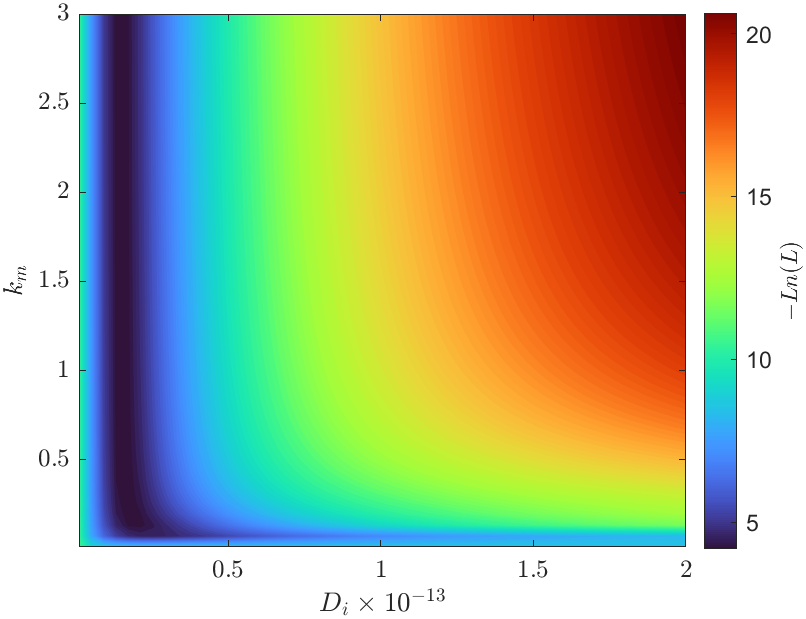
\includegraphics[trim = 0.0cm 0.0cm 0.0cm 0.0cm,clip, width=\columnwidth]{/Results_estimation/Parameter_Space_Linear_Dataset_1.png}
		\caption{The linear kinetic model \\ ~}
		\label{fig: Fit_1_linear}
	\end{subfigure}
	\hfill
	\begin{subfigure}{0.9\columnwidth}
		\centering
		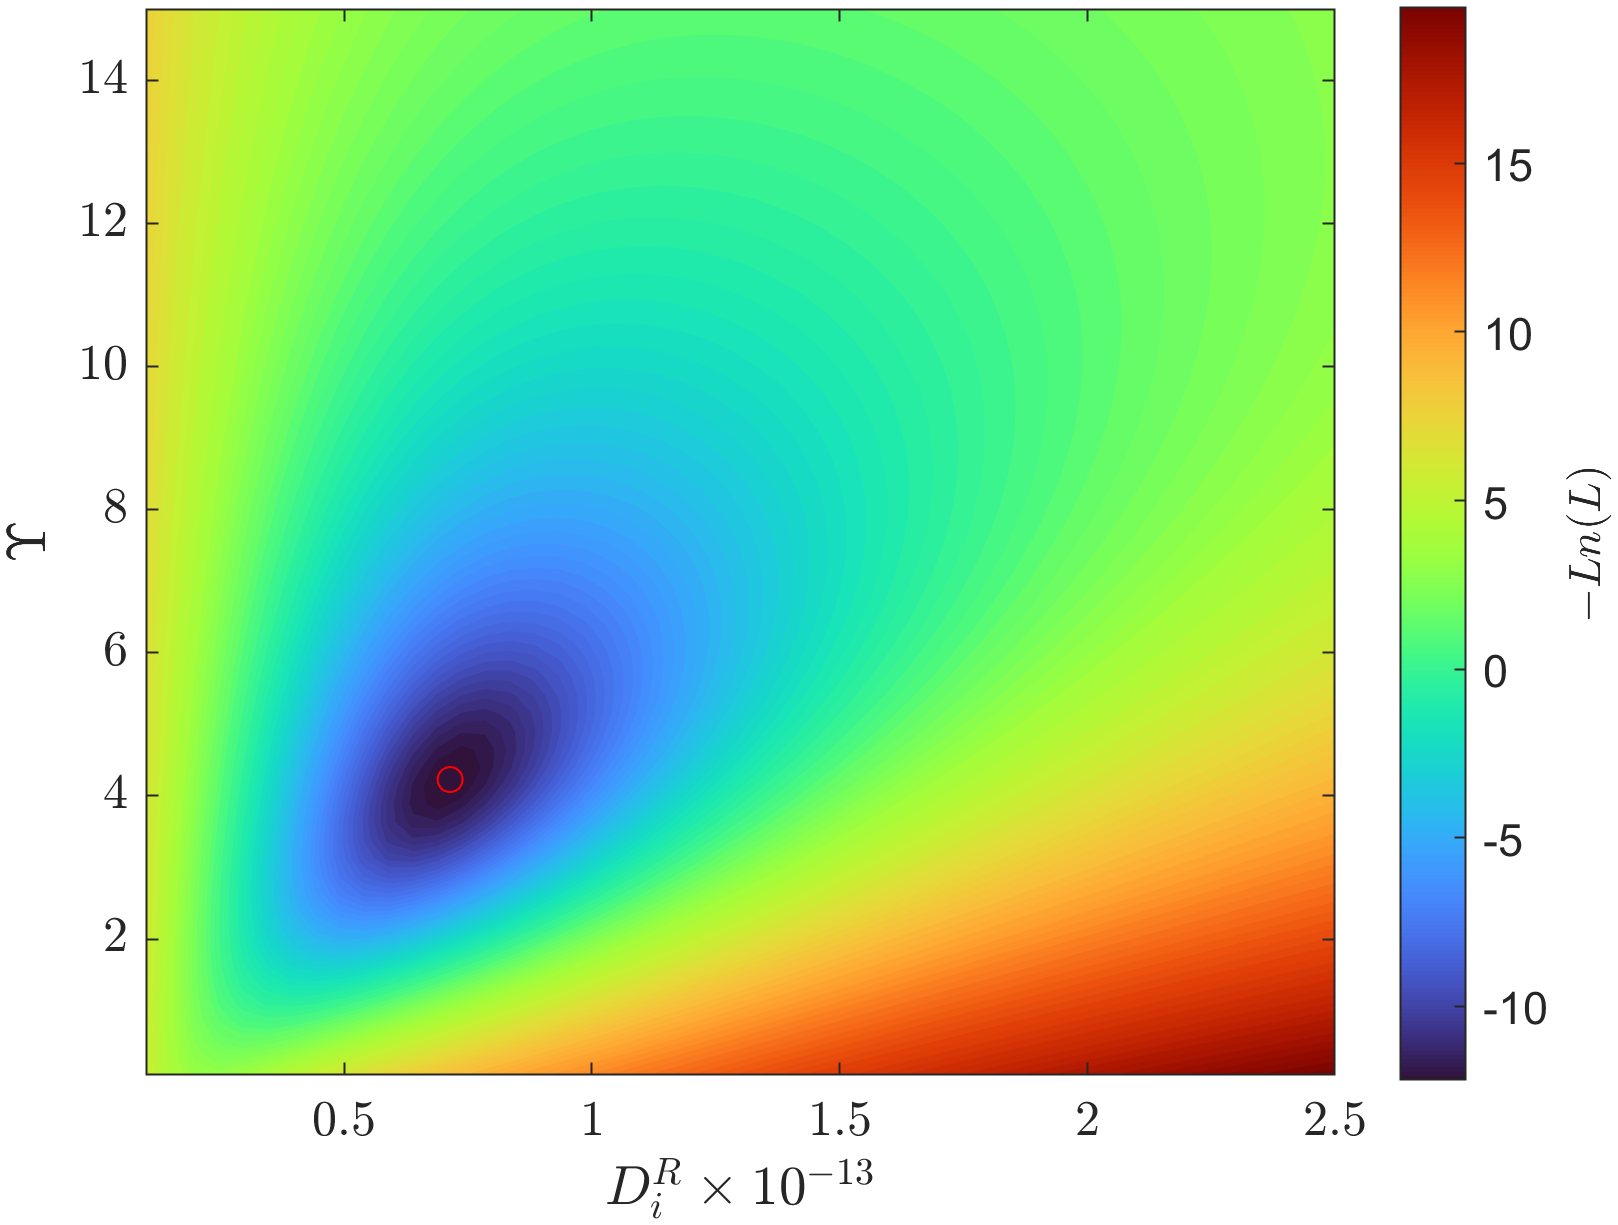
\includegraphics[trim = 0.0cm 0.0cm 0.0cm 0.0cm,clip, width=\columnwidth]{/Results_estimation/Parameter_space_Di_Gamma_dataset_1_org.png}
		\caption{The modified model}
		\label{fig: Fit_1_Di_Gamma}
	\end{subfigure}
	\caption{Parameter space for experiment 1.}
	%\label{fig: Fit_Di_Gamma}
\end{figure}

Figure \ref{fig: Fit_1_linear} shows the parameter space and corresponding values of the cost function for experiment 1 ($40^\circ C$, 100 bar and 6.67$\cdot 10^{-5}$ kg/s). A black-coloured section, in the shape of a vertical stripe at $D_i \approx 0.2$, indicates the minimum values of the cost function $-\ln(L)$. In the direction of $k_m$, the cost function is almost flat, which suggests that any value of $k_m$ above 0.1 fits the data equally well. If $k_m$ can be an arbitrary point, then it can grow to infinity, which suggests that the solvent is far from saturation, and the model can be simplified. The model reduction can be introduced by considering the limit of $k_m$:

{\footnotesize
	\begin{equation*}
		\begin{split}
			&\lim_{k_m \rightarrow \infty} \left({\color{black}{\color{black} c_s} }(t,z)  - \cfrac{{\color{black}\rho_s}}{{\color{black}k_m}(T(t,z)){\color{black}\rho}(T(t,z),{\color{black}P}(t))}  c_f \right)  = \\
			&= \left({\color{black}{\color{black} c_s} }(t,z)  - \cfrac{\rho_s}{\infty \cdot \rho(T(t,z),P(t))}  {c_f}(t,z) \right) = \left(c_s(t,z) - 0 \right)
		\end{split}
\end{equation*} }

In the scenario previously discussed, the fitting outcomes were not deemed satisfactory. Building upon the concepts underlying the Broken-and-Intact and Shrinking Core models (detailed in Section \ref{CH: Gamma_Function}), the $\gamma$ function is introduced to capture the decreasing extraction kinetics. The correction factor is combined with the simplified linear model, resulting in a two-parameter model ($D_i^R$ and $\Upsilon$) as given by Equation \ref{Model_kinetic}. Figure \ref{fig: Fit_1_Di_Gamma} shows the parameter space and the corresponding cost function values.

\begin{figure}[!h]
	\centering
	\begin{subfigure}{0.9\columnwidth}
		\centering
		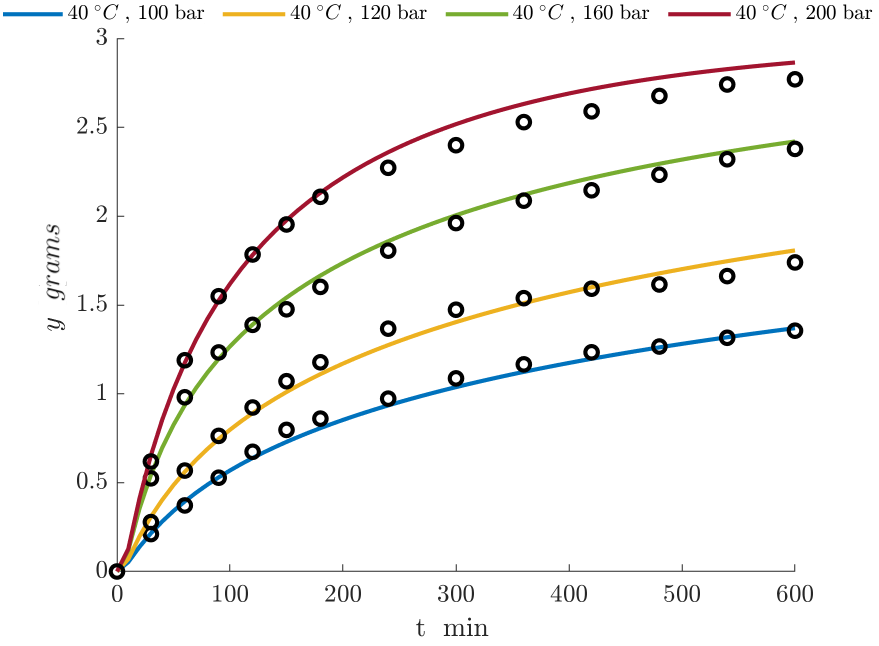
\includegraphics[trim = 0.0cm 0.0cm 0.0cm 0.0cm,clip, width=\columnwidth]{/Results_estimation/Fit_Di_Gamma_1_4_1.png}
		\caption{Parameter estimation results at $6.67\cdot 10^{-5}$ kg/s and temperature of 40 $^\circ C$}
		\label{fig: Fit_1_4_Di_Gamma}
	\end{subfigure}
	\hfill
	\begin{subfigure}{0.9\columnwidth}
		\centering
		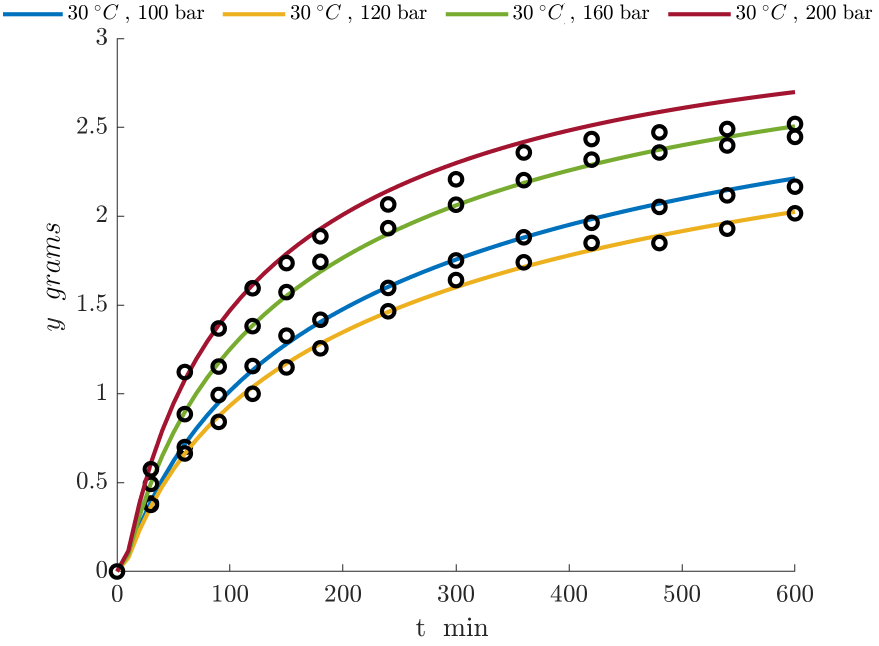
\includegraphics[trim = 0.0cm 0.0cm 0.0cm 0.0cm,clip, width=\columnwidth]{/Results_estimation/Fit_Di_Gamma_5_8_1.png}
		\caption{Parameter estimation results at $6.67\cdot 10^{-5}$ kg/s and temperature of 30 $^\circ C$}
		\label{fig: Fit_5_8_Di_Gamma}
	\end{subfigure}
	\hfill
	\begin{subfigure}{0.9\columnwidth}
		\centering
		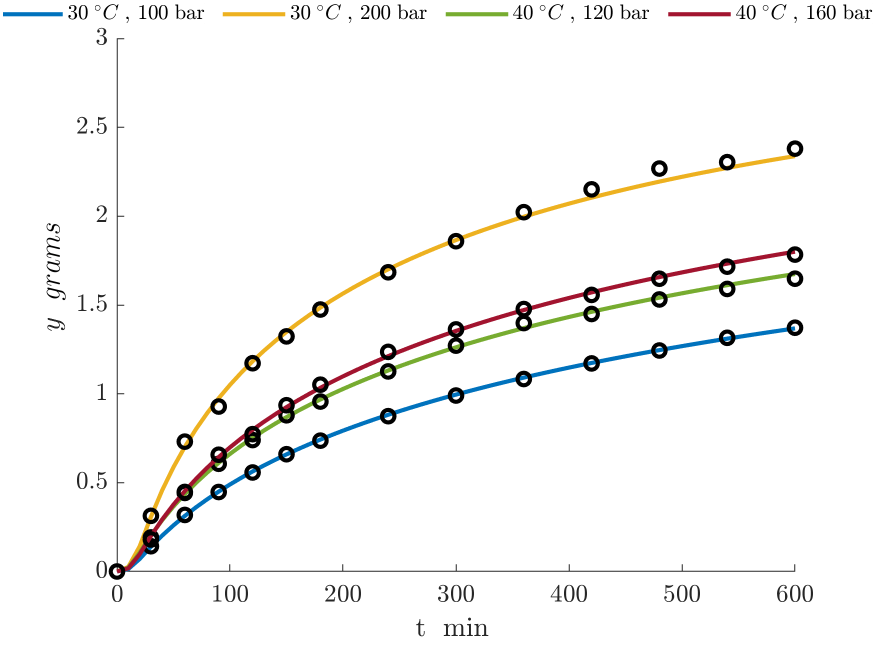
\includegraphics[trim = 0.0cm 0.0cm 0.0cm 0.0cm,clip, width=\columnwidth]{/Results_estimation/Fit_Di_Gamma_9_12_1.png}
		\caption{Results of parameter estimation for experiments at $3.33\cdot 10^{-5}$ kg/s}
		\label{fig: Fit_9_12_Di_Gamma}
	\end{subfigure}
	\caption{Parameter estimation results obtained from the modified model.}
	\label{fig: Fit_Di_Gamma}
\end{figure}

The parameter space for the modified model exhibits a distinct minimum value corresponding to the solution of the parameter estimation problem for experiment 1. The red circle highlights the minimum value of the cost function found by the optimiser. The remaining experiments are fitted to the modified extraction model, and the results, presented in Figure \ref{fig: Fit_Di_Gamma}, show good agreement with the experimental data. 

The parameter estimation results are combined to analyse the relationship between the obtained parameters and the operating conditions. Unlike traditional methods that employ a combination of Reynolds, Schmidt and Sherwood numbers to find correlation, the approach in this study leverages the fixed-bed Reynolds number $\left(Re = \frac{2r \cdot \rho_f \cdot u}{\mu}\right)$ as the sole independent variable. Using the Reynolds number has the advantage of considering the influence of all the control variables (temperature, pressure and flow rate), which means it can be uniquely defined by selecting the operating conditions.	

\begin{figure}[!h]
	\centering
	\begin{subfigure}{0.9\columnwidth}
		\centering
		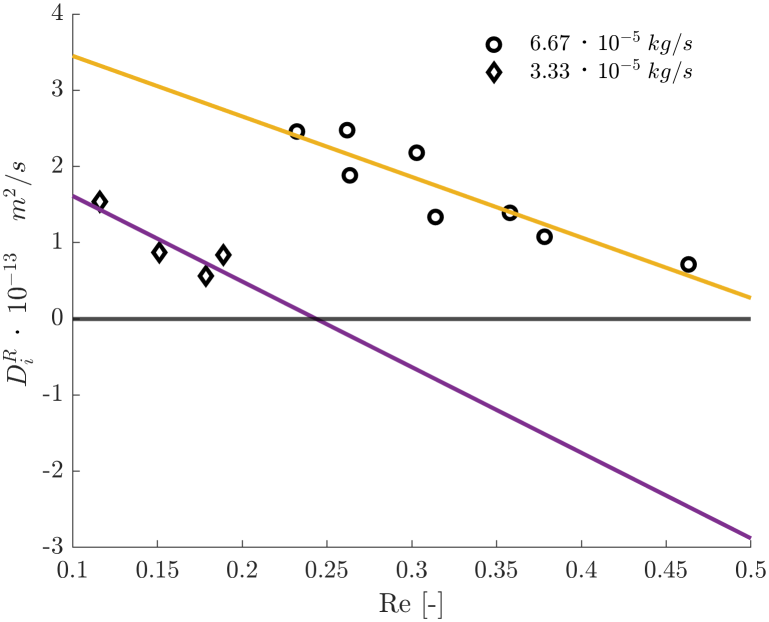
\includegraphics[trim = 0.0cm 0.0cm 0.0cm 0.0cm,clip, width=\columnwidth]{/Results_estimation/Correlation_Di_Re_1.png}
		\caption{Linear regression $D_i^R = f(Re)$}
		\label{fig: Correlations_Di_Re}
	\end{subfigure}
	\hfill
	\begin{subfigure}{0.9\columnwidth}
		\centering
		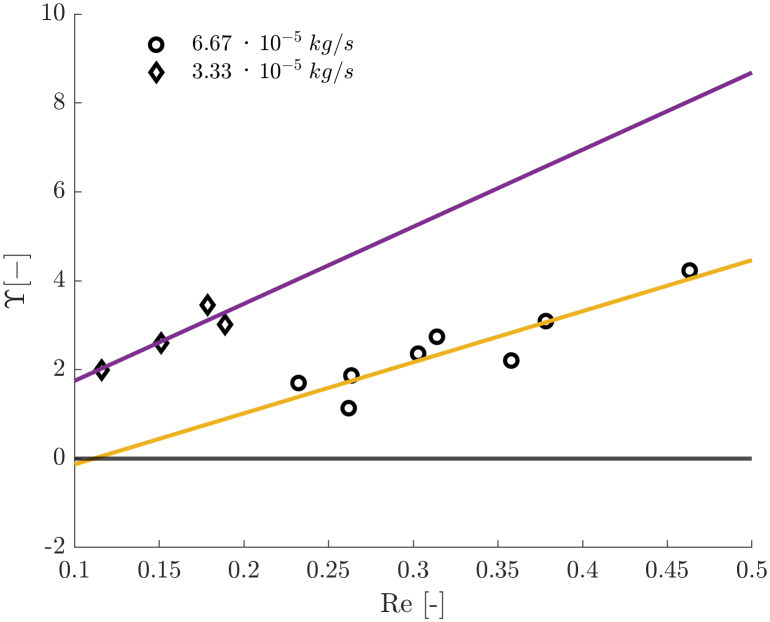
\includegraphics[trim = 0.0cm 0.0cm 0.0cm 0.0cm,clip, width=\columnwidth]{/Results_estimation/Correlation_Gamma_Re_1.png}
		\caption{Linear regression $\Upsilon = f(Re)$}
		\label{fig: Correlations_Gamma_Re}
	\end{subfigure}
	\caption{Linear correlations between parameters.}
	%\label{fig: Correlations_surface}
\end{figure}

In Figures \ref{fig: Correlations_Di_Re} and \ref{fig: Correlations_Gamma_Re}, two distinct data clusters emerge, each corresponding to a different mass flow rate. Despite the linear trends observed in both sets of correlations, the data points for $D_i^R$ decrease with increasing $Re$, while those for $\Upsilon$ increase with $Re$. The reduction of $D_i^R$ with an increase of $Re$ can be attributed to higher fluid density and increased mass transfer resistance.

\begin{figure}[!h]
	\centering
	\begin{subfigure}{0.9\columnwidth}
		\centering
		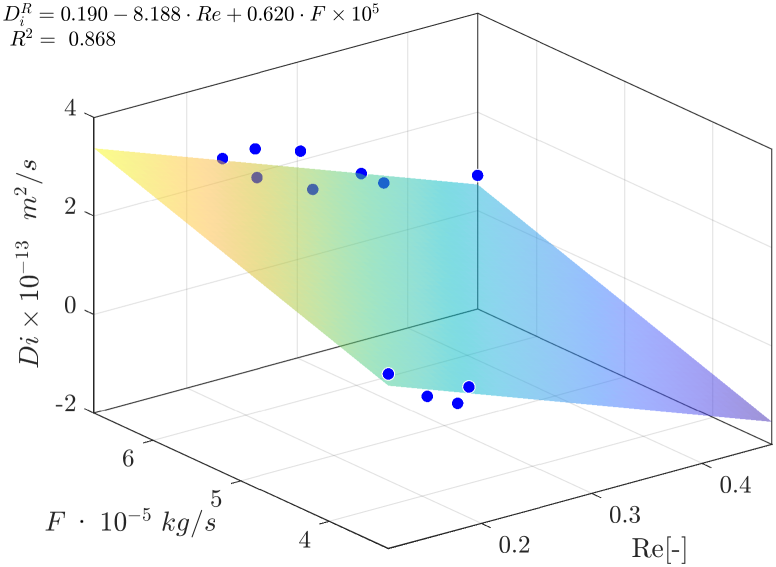
\includegraphics[trim = 0.0cm 0.0cm 0.0cm 0.0cm,clip, width=\columnwidth]{/Results_estimation/Di_Re_F_1.png}
		\caption{Multiple linear regression $D_i^R = f(Re, F)$}
		\label{fig: Correlations_Di_Re_F}
	\end{subfigure}
	\hfill
	\begin{subfigure}{0.9\columnwidth}
		\centering
		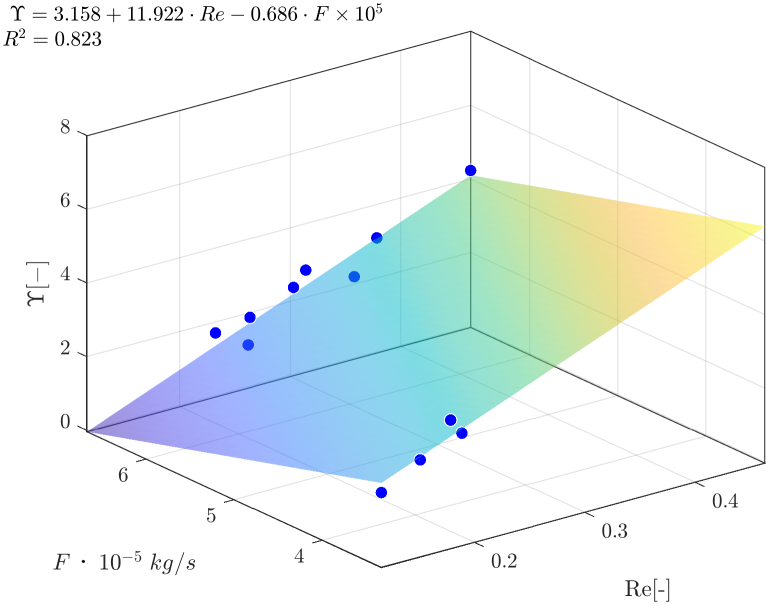
\includegraphics[trim = 0.0cm 0.0cm 0.0cm 0.0cm,clip, width=\columnwidth]{/Results_estimation/Gamma_Re_F_1.png}
		\caption{Multiple linear regression $\Upsilon = f(Re, F)$}
		\label{fig: Correlations_Gamma_Re_F}
	\end{subfigure}
	\caption{Empirical correlations between parameters.}
	%\label{fig: Correlations_surface}
\end{figure}

A more general relationship can be obtained by applying multiple linear regression instead of linear regression. The data clusters in Figure \ref{fig: Correlations_Di_Re} and \ref{fig: Correlations_Gamma_Re} are close to parallel, suggesting that a plane would combine all the data points. The Reynolds number and mass flow rate act as independent variables for $D_i^R$ and $\Upsilon$, as presented in Figures \ref{fig: Correlations_Di_Re_F} and \ref{fig: Correlations_Gamma_Re_F}. The presented correlations are valid in the whole range of investigated operating conditions. The correlations are later tested against the original dataset to show that the correlations can reproduce the results with satisfactory accuracy. Figure \ref{fig: Fit_Di_Gamma_correlation} shows the results of the simulations with incorporated correlations. Good agreement between the simulation results and the dataset can be observed. If Figures \ref{fig: Fit_Di_Gamma} and \ref{fig: Fit_Di_Gamma_correlation} are compared, a decrease in the accuracy of simulations can be observed. Such behaviour is expected due to the bias-variance trade-off, which describes the relationship between a model's complexity and the accuracy of its predictions.

\begin{figure}[!h]
	\centering
	\begin{subfigure}{0.9\columnwidth}
		\centering
		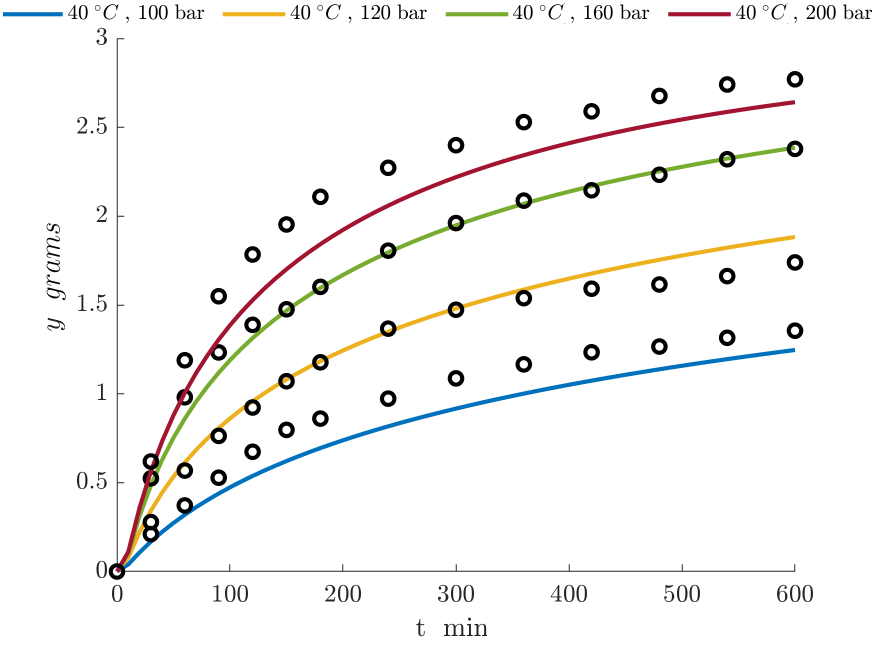
\includegraphics[trim = 0.0cm 0.0cm 0.0cm 0.0cm,clip, width=\columnwidth]{/Results_estimation/Fit_Di_Gamma_1_4_correlation_1.png}
		\caption{Simulation results obtained at $6.67\cdot 10^{-5}$ kg/s and temperature of 40 $^\circ C$}
		\label{fig: Fit_1_4_Di_Gamma_correlation}
	\end{subfigure}
	\hfill
	\begin{subfigure}{0.9\columnwidth}
		\centering
		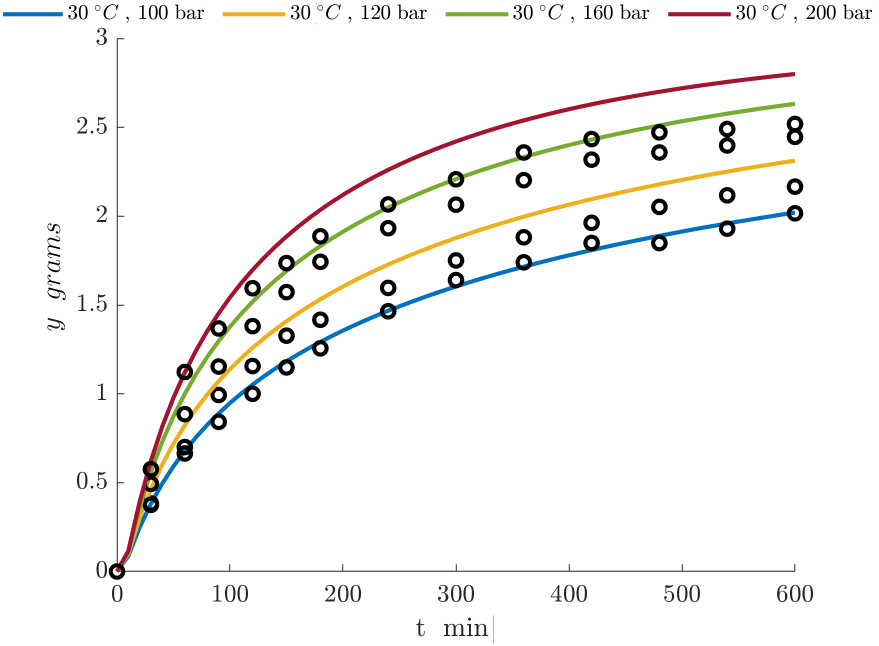
\includegraphics[trim = 0.0cm 0.0cm 0.0cm 0.0cm,clip, width=\columnwidth]{/Results_estimation/Fit_Di_Gamma_5_8_correlation_1.png}
		\caption{Simulation results obtained at $6.67\cdot 10^{-5}$ kg/s and temperature of 30 $^\circ C$}
		\label{fig: Fit_5_8_Di_Gamma_correlation}
	\end{subfigure}
	\hfill
	\begin{subfigure}{0.9\columnwidth}
		\centering
		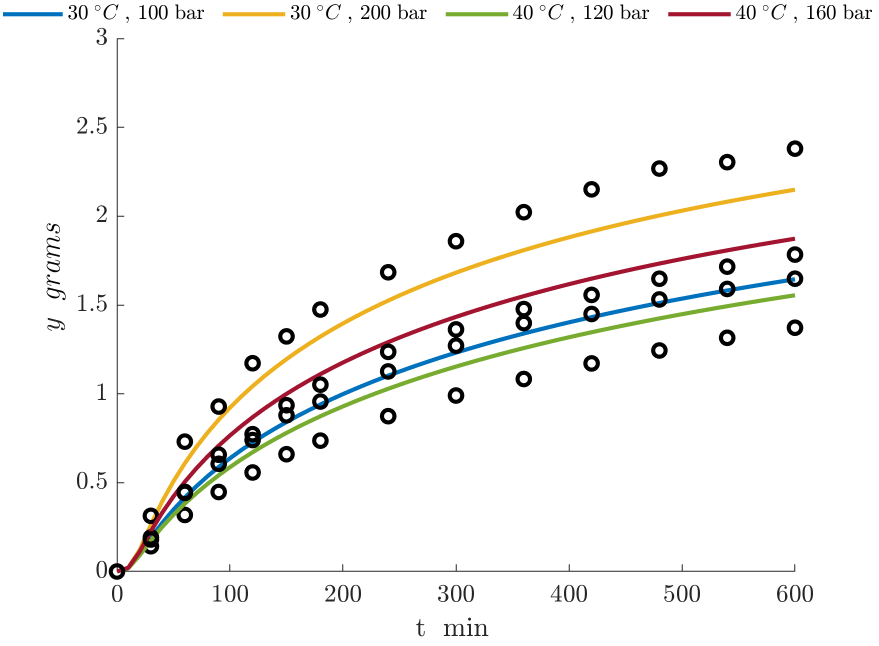
\includegraphics[trim = 0.0cm 0.0cm 0.0cm 0.0cm,clip, width=\columnwidth]{/Results_estimation/Fit_Di_Gamma_9_12_correlation_1.png}
		\caption{Simulation results obtained at $3.33 \cdot 10^{-5}$ kg/s}
		\label{fig: Fit_9_12_Di_Gamma_correlation}
	\end{subfigure}
	\caption{Simulation results from the modified model and correlations}
	\label{fig: Fit_Di_Gamma_correlation}
\end{figure}

The parameter estimation results are compared against those presented by \citet{Povh2001}, who applied the Sovova model to the same dataset. It is important to note that, as the initial solute mass ratio, \citet{Povh2001} used  a value of 10\% above the total amount of extract for every experiment, while in this work, the initial conditions are the same for all the experiments. In contrast to this work, \citet{Povh2001} did not utilise numerical solvers but used a mix of analytical methodologies and trial-and-error procedures. \citet{Povh2001} remarked that 'the direct fitting of experimental data to Sovova's model produced parameters that could not be accepted after a careful physical interpretation of the system'. The parameters identified in this study have a physical interpretation and are within the expected range.

\citet{Rahimi2011} analysed the same dataset using the desorption–dissolution–diffusion model. To decrease the number of unknown parameters, \citet{Rahimi2011} applied a set of empirical correlations. The remaining parameters were determined using a genetic algorithm to solve the parameter estimation problem for each experiment individually. The results obtained by \citet{Rahimi2011} show that the desorption–dissolution–diffusion model fails to reproduce the yield data. The main difference between the model employed by \citet{Rahimi2011} and the one in this study is the $\gamma$ function. The $\gamma$ function increases the model's flexibility by adjusting $D_i$ and allows it to obtain a better fit.

\citet{Povh2001} and \citet{Rahimi2011} delivered a set of independent parameters for every experiment. This work combines the parameters obtained from each experiment to obtain a single correlation valid for the whole range of investigated operating conditions.

% ===================================================
% Section: Conclusion
% ===================================================
\section{Conclusions} \label{CH: Conclusion}

The article has presented a comprehensive study on the supercritical fluid extraction of essential oil from chamomile flowers, focusing on developing and applying a distributed-parameter model to describe the fluid-solid extraction process. By employing the concept of quasi-one-dimensional flow, the study simplifies the spatial dimensions of the extraction process, ensuring uniform flow across any cross-section while allowing for variations in the area available for the fluid phase. The physical properties of the solvent are estimated using the Peng-Robinson equation of state.

The model calibration is based on the data from laboratory experiments conducted by \citet{Povh2001} under various conditions. The model parameters, such as the partition factor, internal diffusion coefficient and decaying factor, were determined through maximum likelihood estimation based on experimental data. The parameter space exploration revealed that while some parameters could be determined with a high degree of confidence, others, like the partition factor, had a low impact on the model's output. The identification of low-impact parameters leads to model reduction. This work introduced a set of correlations to find a general relationship between the parameters and the operating conditions. The obtained correlations were incorporated into the process model and tested against the dataset. The process model is capable of reproducing the dataset with satisfactory accuracy.

The process model can be further used with the presented correlations to introduce an extraction model with dynamically changing operating conditions for multiple purposes, such as yield maximisation, local sensitivity analysis, techno-economic analysis or optimal design of experiments.

% ===================================================
% Bibliography
% ===================================================
%% Loading bibliography style file
%\clearpage
\newpage
%\bibliographystyle{model1-num-names}
\bibliographystyle{unsrtnat}
\bibliography{mybibfile}

\clearpage \appendix \label{appendix}
\section{Appendix} 

%\subsection{Thermodynamic}
%\subfile{Sections/Qubic_EOS} \label{subsubsec: Equation of state}
\label{CH: Thermodynamic_details}

\subsection{Equation of state} \label{subsubsec: Equation of state}

A cubic equation of state (EoS) serves as a mathematical model to describe the behaviour of real gases and liquids through a third-degree polynomial equation that correlates a substance's pressure, volume and temperature. These equations constitute tools for comprehending phase behaviour, properties and thermodynamic processes of real substances across various engineering and scientific applications. The cubic equation of state takes into account deviations from ideal gas behaviour, which are particularly important at high pressures and low temperatures, where real gases do not follow the assumption of an ideal gas.

{\footnotesize
	\begin{equation}
		P = \frac{RT}{v_m-b} - \frac{\Phi}{v_m^2 - ubv_m + wb^2}
	\end{equation}
}

In this equation, $P$ denotes the pressure of the substance, $v_m$ represents the molar volume of the substance, $T$ stands for the absolute temperature of the substance, $u$ and $w$ are integers that vary from one equation to another, $R$ symbolizes the universal gas constant, $\omega$ denotes an acentric factor and $\Phi=a\alpha$.

The Van der Waals constants constitute empirical values contingent upon the particular substance being modelled. These constants factor in molecular interactions (represented by '$a$') and the finite size of gas molecules (indicated by '$b$'). 

Several variations of the cubic equation of state exist, each with its own set of parameters and assumptions. Tables \ref{tab:Popular_Cubic_EoS} and \ref{tab:Popular_Cubic_EoS_alpha} show parameters for popular cubic EoS.

\begin{table}[h!]
	\centering
	\adjustbox{width=0.9\columnwidth}{%
		\begin{tabular}{|c| c c c c|} 
			\hline
			EoS & u & w & a & b\\
			\hline
			van der Waals  & 0 & 0 & $\frac{27}{64} \frac{R^2T_c^2}{P_c}$ & $\frac{RT_c}{8P_c}$ \\
			Redlich and Kwong & 1 & 0 & $0.42748 \frac{R^2T_c^{2.5}}{P_c}$ & $\frac{0.08664RT_c}{P_c}$ \\
			Soave & 1 & 0 & $0.42748 \frac{R^2T_c^2}{P_c}$ & $\frac{0.08664RT_c}{P_c}$ \\
			Peng and Robinson \cite{Peng1976} & 2 & -1 & $0.45724 \frac{R^2T_c^2}{P_c}$ & $\frac{0.07780T_c}{P_c}$\\
			\hline
	\end{tabular} }
	\caption{Parameters for Popular Cubic EoS.}
	\label{tab:Popular_Cubic_EoS}
\end{table}

\begin{table}[h!]
	\centering
	\adjustbox{width=0.9\columnwidth}{%
		\begin{tabular}{|c| c c|} 
			\hline
			EoS & $\alpha$ & f($\omega$)\\
			\hline
			van der Waals  & - & - \\
			Redlich and Kwong & $\frac{1}{\sqrt{T_r}}$ & - \\
			Soave & $\left[ 1 + f(\omega) \left( 1-\sqrt{T_r} \right) \right]^2$ & 0.48+1.574$\omega$-0.176$\omega^2$\\
			Peng and Robinson (\cite{Peng1976}) & $\left[ 1 + f(\omega) \left( 1-\sqrt{T_r} \right) \right]^2$ & 0.37464+1.54226$\omega$-0.26992$\omega^2$ \\
			\hline
	\end{tabular} }
	\caption{Parameters for Popular Cubic EoS.}
	\label{tab:Popular_Cubic_EoS_alpha}
\end{table}

The general cubic equation of state can be represented as a polynomial, as indicated in Equation \ref{EQ:Compressibility_Polynomial}. In a one-phase region, the fluid is characterized by a single real root corresponding to the gas, liquid or supercritical phase. In the two-phase region, a gas-liquid mixture exists, and two roots are identified. The larger root corresponds to the gas phase, while the smaller root pertains to the liquid phase.

{\footnotesize
	\begin{equation}
		\label{EQ:Compressibility_Polynomial}
		Z^3 - (1+B-uB)Z^2+(A+wB^2-uB-uB^2)Z - AB - wB^2 - wB^3 = 0
\end{equation} }

where $A=\frac{\Phi P}{R^2T^2}$ and $B=\frac{bP}{RT}$.

If the Peng-Robinson equation of state (\citet{Peng1976}) is used, the polynomial equation becomes

{\footnotesize
	\begin{equation}
		\label{EQ:Peng_Robinson_Polynomial}
		Z^3 - (1-B)Z^2+(A-2B-3B^2)Z -(AB-B^2-B^3) = 0
\end{equation} }

For an ideal gas, the compressibility factor is defined as $Z = 1$, but the deviation of Z needs to be considered for real-life cases. The value of $Z$ typically increases with pressure and decreases with temperature. At elevated pressures, molecules collide more frequently, which allows the repulsive forces between molecules to influence the molar volume of the real gas ($v_m$), making it surpass that of the corresponding ideal gas $\left( \left(v_m\right)_{ideal~gas} = \frac{RT}{P} \right)$, resulting in $Z$ exceeding one. At lower pressures, molecules move freely, with attractive forces predominating, leading to $Z < 1$.

Numerical methods such as Newton-Raphson can be used to solve the polynomial equation to obtain the compressibility $Z\left(T(t,z), P(t)\right)$ at a given temperature and pressure. Alternatively, a closed-form solution can be obtained by using the Cardano formula (Appendix \ref{CH: Cardano}).

\subsubsection{Density of the fluid phase} \label{subsubsec: Fluid density}

The density of the fluid can be calculated from the real gas equation $\rho = \frac{P}{RTZ} \frac{1}{m_{CO2}}$. The temperature can be obtained from the time evolution of governing equations, and the pressure is considered to be constant along the system. 


\subsection{Cardano's Formula} \label{CH: Cardano}

Following the work of \citet{Gmehling2019}, a cubic equation of state can be written in the following form:

{\footnotesize
	\begin{equation}
		Z^3 + UZ^2+ SZ + T = 0
	\end{equation}
}

where Z is the compressibility factor. Cubic equations can be solved analytically using Cardano's formula:

{\footnotesize
	\begin{equation*}
		P = \cfrac{3S-U^2}{3} \qquad Q = \cfrac{2U^3}{27}-\cfrac{US}{3} + T
	\end{equation*}
}

The discriminant can be determined to be

{\footnotesize
	\begin{equation}
		D = \left( \cfrac{P}{3} \right)^3 + \left( \cfrac{Q}{2} \right)^2
	\end{equation}
}

For $D>0$, the equation of state has one real solution:

{\footnotesize
	\begin{equation}
		Z = \left[ \sqrt{D} - \cfrac{Q}{2} \right]^{1/3} - \cfrac{P}{ 3 \left[ \sqrt{D}-\cfrac{Q}{2} \right]^{1/3} } - \cfrac{U}{3}
	\end{equation}
}

For $D<0$, there are three real solutions:

{\footnotesize
	\begin{equation*}
		\Theta = \sqrt{-\cfrac{P^3}{27}} \qquad \Phi = \arccos\left( \cfrac{-Q}{2\Theta} \right)
	\end{equation*}
}

They can be written as

{\footnotesize
	\begin{align}
		Z_1 &= 2\Theta^{(1/3)} \cos \left( \cfrac{\Phi}{3} \right) - \cfrac{U}{3} \\
		Z_2 &= 2\Theta^{(1/3)} \cos \left( \cfrac{\Phi}{3} + \cfrac{2\pi}{3} \right) - \cfrac{U}{3} \\
		Z_3 &= 2\Theta^{(1/3)} \cos \left( \cfrac{\Phi}{3} + \cfrac{4\pi}{3} \right) - \cfrac{U}{3} 
	\end{align}
}

The largest and smallest are the vapour and liquid phases, respectively. The middle one has no physical interpretation.

\end{document}